\section{The feature computation update mechanism.}
\label{sec:FeatureComputationUpdateMechanism}

In this chapter we explain one of the important aspect of feature computation in Mastodon, in the case of large data.
As we repeated several times in this manual, Mastodon is meant to harness large images and large data generated from it. 
You probably noticed that the feature computers that deal with spot intensity (\texttt{Spot gaussian-filtered intensity}, \texttt{Spot median intensity}, \texttt{Spot sum intensity}) were taking a long time to compute. 
They require synchronized access to pixel data, jumping from one spot to another, at a fixed resolution level.
In situations where you have millions of spots, the computation of these features will take a very long time, possibly similar to the time it took to detect these spots. 
So of course, you don't want to do it again and again each time one spot changes radius or position.
You want to recompute feature values only for the spots that have been altered or created since the last computation. 
An added complication is that sometimes the user might chose not to compute a certain feature, but we still need to keep track of the changes since this feature has been computed, independently of others.

Mastodon has a system that supports incremental updates. 
This system tracks what data items have been modified or created for a given number of feature computation times. 
It can provide to the feature computer that request it the list of data items that changed since the feature it provides have been last computed.
This system is based on an \textit{update stack} of \texttt{UpdateState}s, and each \texttt{UpdateState} stores:
\begin{itemize}
    \item the list of the names of features that were computed in the last computation. 
    Later in this chapter they are referred as \textbf{keys} of the update state.
    \item and the collection of data items (spots and links) that were added or modified since this last computation. This collection is called the \textbf{value} of the update state.
\end{itemize}
\noindent There are two stacks, one for spots, one for links.
They have a limited size, so that they can "forget" about ancient computation events. 

To illustrate how it works, let us consider two features \textbf{A} and \textbf{B} that are defined on spots.
On the example described in Figure~\ref{fig:FeatureUpdateStack}, at \textit{t0} the features are not computed. 
We have a model made of two spots \textit{s1} and \textit{s2} connected by a link.
The update stack is initialized with a single item with an empty \texttt{UpdateState}.

At $t_1$, the user triggers a computation of both features \textbf{A} and \textbf{B}. 
Because none of the feature names for \textbf{A} and \textbf{B} can be found in the update stack, a computation of the feature values for all the spots of the model is triggered.

At $t_2$, once the computation is finished, a new update item is pushed on stack. 
It is initialized with an empty collection for value, and the name of the features that were calculated (\textbf{A} and \textbf{B}) are stored as key.

At $t_3$ the user moves the spot \textit{s1}. 
Because there are some listeners wired to the update stack, \textit{s1} is added to the value collection of the top item in the stack. 
That is: the one with \textbf{A} and \textbf{B} names as key that was created after \textbf{A} and \textbf{B} computation. 
Both features \textbf{A} and \textbf{B} are marked as not up-to-date.

At $t_4$ the user triggers the computation of feature \textbf{A} only. 
Since the feature computer for \textbf{A} uses incremental feature update, it queries the changes for its feature. 
This call does the following:

\begin{itemize}
    \item  The method iterates through the update stack items, top to bottom.
    
    \item The first update item is inspected for its key. 
    The key is a collection of feature names.
    
    \item Since the first key contains the feature name for \textbf{A}, iteration stops, and the call returns the value of this item.
    
    \item This value is a collection simply made of the spot \textit{s1}, so the feature computer recompute the feature value only for \textit{s1}.

\end{itemize}

At $t_5$, after computation, a new update item is added to the update stack. Since we computed only \textbf{A}, its key contains only the name of \textbf{A}. 
As before, the item is initialized with an empty collection as value. 
\textbf{A} is marked up-to-date.

At $t_6$ the user moves the spot \textit{s2}. 
As before, it is added to the value collection of the top item in the stack. 
This time, it is the one with the name of \textbf{A} as key.

Now at $t_7$ the user wants to compute feature \textbf{B}, which is not up-to-date since $t_2$. 
Again, the feature computer for \textbf{B} uses incremental feature computation. 
The call does the following:

\begin{itemize}

    \item The method iterates through the update stack items, top to bottom.
    
    \item The first update item does not contain the name of \textbf{B}, so we move down to the next item.
    
    \item The second item contains the name of \textbf{B}. We stop there.
    
    \item Now that we need to return the collection of spots to update, we iterate back to the first item, bottom to top:
    
    \begin{itemize}
        \item First we take the collection of spots for the second item: \textit{s1}.
        \item  Then we move up to the first update item in the stack, that contains \textit{s2}, and concatenate with it. 
        We end up with a collection made of { \textit{s1}, \textit{s2} }.
    \end{itemize}

    \item We recompute \textbf{B} only for \textit{s1} and \textit{s2} which makes it up-to-date.
\end{itemize}
\noindent After this computation ($t_8$) a new update item is pushed to the update stack, with the name of \textbf{B} as key.

And it goes on like this. 
If after the steps exemplified here the user would recompute all features, the changes for \textbf{B} would be empty, and the changes for \textbf{A} would be built by iterating to the second item in the stack, that contains only \textit{s2}.

You can it a try with a larger dataset than the one we have been using so far.
Compute all the features, including the costly ones such as \texttt{Spot gaussian-filtered intensity}.
The first time you compute this features, it should take a significant amount of time.
Now move one spot from one position to another, and recompute all the features. 
You should see that now the computation takes much less time.

\begin{figure}
    \centering
    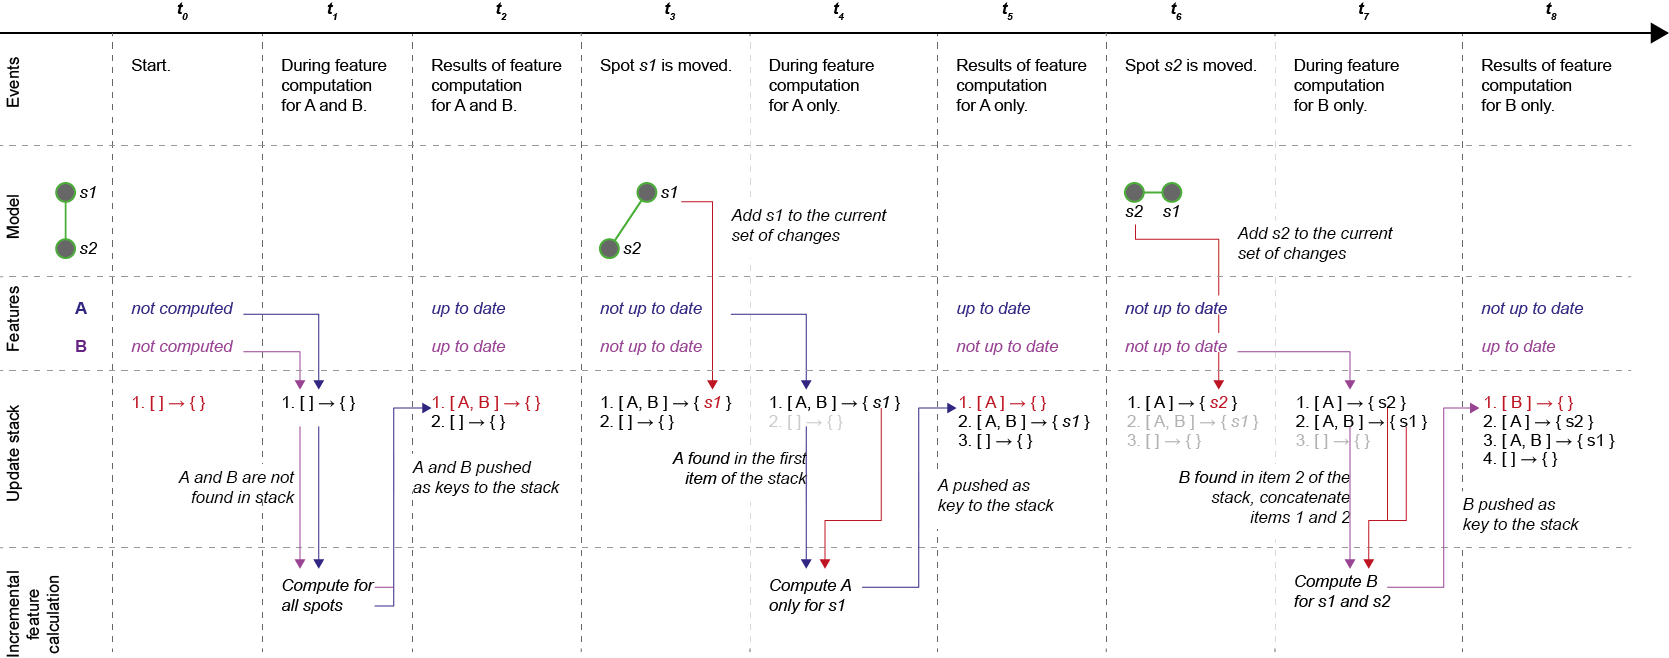
\includegraphics[angle=90, height=0.8\textheight]{figures/Mastodon_FeatureUpdateStack.png}
    \caption{An illustration of the feature update stack mechanism.  }
    \label{fig:FeatureUpdateStack}
\end{figure}
